\documentclass[a4paper,12pt]{article}

% ---------- Packages ----------
\usepackage[utf8]{inputenc}
\usepackage[T1]{fontenc}
\usepackage[margin=2.5cm]{geometry}
\usepackage{amsmath}
\usepackage{amssymb}
\usepackage{graphicx}
\usepackage{booktabs}
\usepackage{longtable}
\usepackage{array}
\usepackage{xcolor}
\usepackage{hyperref}
\usepackage{url}
\usepackage{cite}
\usepackage{caption}
\usepackage{subcaption}
\usepackage{listings}
\usepackage[protrusion=true,expansion=false]{microtype}
\usepackage{setspace}
\usepackage{fancyhdr}
\usepackage{titlesec}
\usepackage{abstract}
\usepackage{parskip}
\usepackage{float}
\usepackage{multirow}
\newcommand{\doi}[1]{\href{https://doi.org/#1}{doi:{#1}}}
\usepackage{siunitx}
\usepackage{pgfplots}
\pgfplotsset{compat=1.18}

\hypersetup{
  colorlinks=true,
  linkcolor=blue!60!black,
  citecolor=green!50!black,
  urlcolor=blue!70!black,
  pdftitle={Benchmarking FASTQ Quality Control Tools on ARM HPC Hardware with GPU Acceleration},
  pdfauthor={},
}

\lstset{
  basicstyle=\ttfamily\small,
  breaklines=true,
  frame=single,
  backgroundcolor=\color{gray!10},
}

\pagestyle{fancy}
\fancyhf{}
\rhead{\small FASTQ QC Benchmarking on ARM + A100}
\lhead{\small \textit{PhD Research}}
\cfoot{\thepage}

\onehalfspacing

% ---------- Title ----------
\title{%
  \large \textbf{Benchmarking FASTQ Quality Control Tools on ARM HPC Hardware\\
  with GPU Acceleration: A Comparative Performance Study}\\[1em]
  \normalsize \textit{Prepared as part of doctoral research}
}
\author{
  [Author Name]\\
  \small [Department, Institution]\\
  \small [Email]
}
\date{March 2026}

% ===========================================================================
\begin{document}
% ===========================================================================

\maketitle
\thispagestyle{fancy}

% ---------- Abstract ----------
\begin{abstract}
\noindent
Quality control (QC) of raw sequencing data in FASTQ format is an obligatory
first step in virtually every genomics analysis pipeline.  As sequencing
throughput continues to grow, the computational cost of QC has become a
non-trivial bottleneck, motivating both algorithmic improvements and hardware
acceleration.  In this study we perform a systematic performance benchmarking
of four widely used FASTQ QC tools---\textbf{FastQC}, \textbf{Falco}, and two
builds of \textbf{fastp} (the canonical OpenGene release and a GPU-augmented
fork by d0bromir)---on a high-performance computing (HPC) node equipped with a
128-core ARM Neoverse N1 processor and two NVIDIA A100-80GB GPUs.  We evaluate
wall-clock runtime across four real sequencing datasets ranging from 148\,MB to
9.5\,GB in compressed size, sweeping thread counts from 1 to 32.  Our results
show that Falco achieves 1.7$\times$ speedup over FastQC in single-threaded
operation; that fastp scales efficiently to 8 threads for large whole-genome
sequencing (WGS) files before becoming I/O-bound; and, critically, that
post-hoc GPU kernel optimisations (warp-per-read kernel, $16\times$ larger
batch size, concurrent 8-slot dispatch pool) reduce the GPU-enabled fastp fork
wall-clock time by 17.6\% on WGS-6G (105.8\,s\,$\to$\,87.3\,s at
32\,threads), achieving effective parity with the CPU-only path.  We discuss
implications for pipeline design on modern ARM-based HPC infrastructure.

\medskip
\noindent\textbf{Keywords:} FASTQ; quality control; benchmarking; ARM; NVIDIA
A100; GPU acceleration; bioinformatics pipeline; fastp; Falco; FastQC.
\end{abstract}

\newpage
\tableofcontents
\newpage

% ===========================================================================
\section{Introduction}
% ===========================================================================

The rapid decline in sequencing costs associated with second-generation
(Illumina) platforms has led to an explosion in the volume of raw sequencing
data produced annually.  A single NovaSeq 6000 flow-cell can generate in excess
of 6\,Tbp of raw reads per run~\cite{Illumina2023NovaSeq}, and large
population-scale cohorts such as UK Biobank regularly produce petabase-scale
datasets~\cite{Bycroft2018UKBiobank}.  Before any analysis---read alignment,
variant calling, expression quantification---raw reads must be assessed for
technical artefacts introduced during library preparation and sequencing.  This
first step is universally referred to as \emph{quality control} (QC).

While QC is conceptually straightforward, its computational cost scales linearly
with data volume.  In automated pipelines executed across thousands of samples,
the aggregate QC burden is significant.  Historically, FastQC has been the
default tool~\cite{Andrews2010FastQC}, offering rich HTML reports and wide
adoption.  More recent tools such as Falco~\cite{deSenaBrandine2021Falco} and
fastp~\cite{Chen2018fastp} achieve substantial speedups through algorithmic
improvements (Falco) or combined QC-plus-trimming in a streaming single-pass
design (fastp).

Simultaneously, the HPC landscape is diversifying.  ARM-architecture servers
(e.g.\ Ampere Altra, AWS Graviton, Fujitsu A64FX) now routinely appear in
Top-500 lists and cloud offerings, offering competitive performance-per-watt
relative to x86 counterparts~\cite{Ditzel2020ARM}.  GPU co-processors, long
dominant in machine-learning workloads, are being evaluated for genomics
acceleration~\cite{Houtgast2018GPU, Shajii2016Seq}.  The interplay of these
architectural trends has not been systematically evaluated for FASTQ QC tools.

This paper makes the following contributions:
\begin{itemize}
  \item A rigorous, reproducible benchmark of four FASTQ QC tools on a
    128-core ARM Neoverse N1 server with NVIDIA A100 GPUs, spanning
    multi-threaded CPU scaling and GPU-accelerated operation.
  \item Empirical characterisation of the I/O bottleneck that limits CPU
    thread scaling beyond 8 threads for large WGS files.
  \item Experimental evidence that the initial GPU-augmented fastp fork
    incurs overhead on this hardware profile, together with an iterative
    optimisation study (warp-per-read kernel, 16$\times$ batch size,
    concurrent slot pool) that eliminates that overhead and achieves
    GPU\/CPU parity at 32\,threads.
  \item Implementation of a GPU-accelerated BGZF decompressor via the
    NVIDIA nvCOMP batched DEFLATE API, providing a pathway to full I/O
    pipeline GPU acceleration for BGZF-format genomics data.
  \item Practical recommendations for QC pipeline design on ARM HPC nodes.
\end{itemize}

% ===========================================================================
\section{Background: FASTQ Files and Quality Control}
\label{sec:background}
% ===========================================================================

\subsection{The FASTQ Format}

FASTQ is the \emph{de facto} standard file format for storing high-throughput
sequencing reads together with their per-base quality scores~\cite{Cock2010FASTQ}.
Each sequencing read is represented as a four-line record:

\begin{lstlisting}
@SRR123456.1 1 length=150
ACGTACGTACGT...       (nucleotide sequence, length L)
+
IIIIIIIIIIII...       (ASCII-encoded Phred quality scores, length L)
\end{lstlisting}

Phred quality scores $Q$ encode the base-call error probability $p$ as
$Q = -10\,\log_{10}(p)$.  Modern Illumina instruments encode these in ASCII
offset 33 (Sanger/Phred+33 encoding)~\cite{Cock2010FASTQ}.  A score of
$Q30$ corresponds to a 1-in-1000 error rate; $Q20$ to 1-in-100.

FASTQ files are almost universally stored gzip-compressed (\texttt{.fastq.gz}),
yielding compression ratios of approximately 4:1 to 6:1 for typical short-read
data.  Decompression therefore represents a significant fraction of the
wall-clock time of any FASTQ-processing tool.

\subsection{Quality Control Metrics}

QC tools typically compute and report the following metrics:

\begin{itemize}
  \item \textbf{Per-base sequence quality}: distribution of Phred scores at
    each cycle position.  Degraded quality at read tails is normal and expected.
  \item \textbf{Per-sequence quality distribution}: overall quality histogram;
    bi-modal distributions suggest mixed sample quality.
  \item \textbf{Per-base sequence content}: fraction of A/C/G/T at each
    position.  Biases early in the read indicate library preparation artefacts.
  \item \textbf{GC content}: per-read and per-position GC fraction compared to
    a theoretical normal distribution; deviation suggests contamination or bias.
  \item \textbf{Sequence duplication levels}: duplicate fractions estimated by
    hashing read subsets; elevated rates suggest PCR over-amplification.
  \item \textbf{Overrepresented sequences}: detection of adapter sequences,
    rRNA, PhiX spike-in, or other contaminants.
  \item \textbf{Adapter content}: systematic detection of common sequencing
    adapters (Illumina TruSeq, Nextera, etc.).
  \item \textbf{Poly-X content}: homopolymer runs (particularly poly-G) are
    artefacts of two-channel Illumina chemistry (NovaSeq, NextSeq) and
    require trimming.
\end{itemize}

\subsection{Quality Trimming vs.\ QC-Only Operation}

Tools differ in whether they \emph{only report} quality metrics (FastQC, Falco)
or additionally \emph{trim and filter} reads in-place (fastp).  QC-only tools
are read-only and write only an HTML/text report.  Trimming tools modify the
data stream and write a new, cleaned FASTQ file.  fastp operates in a
single-pass streaming mode: it reads, trims, optionally corrects, and writes
while simultaneously accumulating statistics for its report.  This design
typically yields higher throughput than sequential QC-then-trim pipelines.

% ===========================================================================
\section{Software Tools}
\label{sec:tools}
% ===========================================================================

\subsection{FastQC}
\label{sec:fastqc}

FastQC~\cite{Andrews2010FastQC} is the most widely cited FASTQ QC tool,
referenced in tens of thousands of genomics publications.  It is written in
Java and processes each read sequentially, accumulating statistics using a set
of analysis modules.  The tool supports optional multi-file parallelism via its
\texttt{-t~N} flag, which allocates one thread per input file but does not
parallelize within a single file.  FastQC produces well-formatted HTML reports
with embedded plots and a \texttt{PASS}/\texttt{WARN}/\texttt{FAIL} summary.
We built FastQC from source (s-andrews/FastQC, GitHub) using Apache Ant and
OpenJDK 21.

\subsection{Falco}
\label{sec:falco}

Falco~\cite{deSenaBrandine2021Falco} is a C++ re-implementation of FastQC that
is API-compatible (same HTML output format, same flags) but substantially
faster.  It exploits data locality and avoids Java JVM overhead, and is compiled
with aggressive optimisation.  Falco is strictly single-threaded per file;
it does not support intra-file parallelism.  In our tests Falco was compiled
with \texttt{-O3~-march=native} targeting the Neoverse N1 microarchitecture.

\subsection{fastp (OpenGene)}
\label{sec:fastp-og}

fastp~\cite{Chen2018fastp} is a streaming FASTQ preprocessor that performs QC
and trimming in a single pass.  Its C++ implementation uses a producer-consumer
thread model: one thread decompresses and reads, $N{-}2$ worker threads process
reads, and one thread writes.  fastp supports adapter trimming, per-read quality
filtering, sliding-window quality trimming, poly-G detection, UMI handling, and
duplication estimation.  It writes compressed FASTQ output alongside JSON and
HTML reports.  Thread count is controlled via \texttt{-w~N} (worker threads;
total threads including I/O equals $N+2$).  In our tests we benchmarked output
directed to \texttt{/dev/null} to isolate processing time from write bandwidth.

\subsection{fastp (d0bromir GPU fork)}
\label{sec:fastp-gpu}

d0bromir/fastp is an experimental fork of fastp that augments it with CUDA GPU
kernels for quality statistics accumulation, poly-G detection, and sliding-window
trimming.  When CUDA is available, computationally intensive per-read operations
are offloaded to both GPUs via CUDA streams using a round-robin device selector;
the host CPU manages I/O and orchestration.  Our build initialises
\texttt{CudaStatsWrapper} instances for Device~0 and Device~1 at startup and
dispatches batches alternately, achieving verified utilisation of both A100
cards.  The repository (d0bromir/fastp, GitHub) targets Compute
Capability 8.0+ (Ampere architecture, matching our A100 GPUs).  We built both
a CPU-only binary (\texttt{fastp\_d0bromir\_cpu}, compiled without CUDA) and a
GPU-enabled binary (\texttt{fastp\_d0bromir\_gpu}) from the same source tree.

During this study we performed three iterative optimisations of the GPU path
(commits \texttt{1669e38} and \texttt{9dc7631} on d0bromir/fastp):
\begin{enumerate}
  \item \textbf{Warp-per-read kernel:} Replaced the original one-thread-per-read
    CUDA kernel with a 32-thread warp cooperative reduction, improving SM
    occupancy from ${\sim}4$\% to ${\sim}32$\% on the A100.
  \item \textbf{$16\times$ larger batch size:} Increased \texttt{PACK\_SIZE}
    from 512 to 8\,192 reads per batch, amortising kernel launch latency and
    reducing thread-synchronisation overhead (benefiting both GPU and CPU-forced
    code paths).
  \item \textbf{8-slot concurrent dispatch pool:} Replaced the 2-slot blocking
    pool with an 8-slot non-blocking pool to overlap PCIe transfers with kernel
    execution on both GPUs simultaneously.
  \item \textbf{GPU BGZF decompressor (nvCOMP):} Implemented a GPU-accelerated
    BGZF decompressor using the NVIDIA nvCOMP batched DEFLATE API
    (\texttt{nvcompBatchedDeflateDecompressAsync}).  The implementation
    auto-detects BGZF headers (18-byte probe), strips the gzip wrapper to
    expose raw DEFLATE payloads, and decompresses up to 256 blocks (${\le}16$\,MB)
    per dispatch.  Standard gzip input falls back to CPU igzip automatically.
\end{enumerate}

\noindent The quantitative impact of these optimisations is characterised in
Section~\ref{sec:scaling} and Section~\ref{sec:discussion}.

\paragraph{Build challenges on aarch64 / glibc 2.41.}
Compiling the GPU fork on our platform required resolving an incompatibility
between CUDA 13.1 and glibc 2.41 (Ubuntu 25.10): glibc's
\texttt{bits/mathcalls.h} declares \texttt{rsqrt()} and \texttt{rsqrtf()} with
\texttt{noexcept(true)}, while CUDA's \texttt{crt/math\_functions.h} declares
the same symbols without a \texttt{noexcept} specifier.  The C++ standard
prohibits re-declaration with incompatible exception specifications.  We
resolved this by patching the CUDA system header to add the matching
\texttt{noexcept} qualifier, and used GCC 13.4 as the CUDA host compiler
(\texttt{-ccbin~g++-13}) since the default GCC 15.2 was not yet supported by
the CUDA 13.1 driver C++ front-end.

% ===========================================================================
\section{Hardware and Software Environment}
\label{sec:hardware}
% ===========================================================================

\subsection{Compute Node}

All experiments were performed on a single server node configured as described
in Table~\ref{tab:hardware}.

\begin{table}[H]
  \centering
  \caption{Hardware configuration of the benchmark node.}
  \label{tab:hardware}
  \begin{tabular}{ll}
    \toprule
    \textbf{Component} & \textbf{Specification} \\
    \midrule
    Architecture       & ARM AArch64 \\
    CPU microarch      & ARM Neoverse N1 (implementer 0x41, part 0xd0c) \\
    Logical cores      & 128 \\
    System RAM         & 246\,GiB \\
    GPU(s)             & 2 $\times$ NVIDIA A100-SXM4 80\,GB PCIe \\
    GPU compute cap.   & Compute Capability 8.0 (Ampere) \\
    GPU VRAM           & 80\,GB HBM2e per device \\
    Storage            & /dev/md0 software RAID, 893\,GB total, 562\,GB available \\
    \midrule
    OS                 & Ubuntu 25.10 (Oracular Oriole), aarch64 \\
    Kernel             & Linux 6.17.0-14-generic \\
    NVIDIA Driver      & 590.48.01 \\
    CUDA Toolkit       & 13.1 \\
    GCC (default)      & 15.2.0 \\
    GCC (CUDA host)    & 13.4.0 \\
    Java               & OpenJDK 21 \\
    \bottomrule
  \end{tabular}
\end{table}

\subsection{Software Versions and Build Configuration}

All tools were built from source to ensure architecture-specific optimisation.
Table~\ref{tab:versions} summarises the software versions and key build flags.

\begin{table}[H]
  \centering
  \caption{Software versions and build configuration.}
  \label{tab:versions}
  \begin{tabular}{llll}
    \toprule
    \textbf{Tool} & \textbf{Version / Commit} & \textbf{Language} & \textbf{Key build flags} \\
    \midrule
    FastQC            & 0.12.1                  & Java     & \texttt{ant build} \\
    Falco             & 1.2.4                   & C++      & \texttt{-O3 -march=native} \\
    fastp (OpenGene)  & 0.23.4                  & C++      & \texttt{-O3 -march=native}; libisal, libdeflate \\
    fastp (d0bromir, CPU)  & 1.2.2              & C++      & as above, \texttt{WITH\_CUDA=0} \\
    fastp (d0bromir, GPU)  & 1.2.2              & C++/CUDA & \texttt{WITH\_CUDA=1}; \texttt{-gencode arch=compute\_80}; \texttt{-ccbin g++-13} \\
    \bottomrule
  \end{tabular}
\end{table}

\noindent
fastp (both variants) was linked against Intel ISA-L (\texttt{libisal}) for
SIMD-accelerated decompression and libdeflate for deflate operations, both
compiled with \texttt{-march=native} to exploit ARM SVE/NEON vector
instructions available on the Neoverse N1.

% ===========================================================================
\section{Input Data}
\label{sec:data}
% ===========================================================================

\subsection{Dataset Description}

We benchmarked against four real sequencing datasets representing two distinct
data regimes: a small targeted-panel run and three large whole-genome
sequencing (WGS) runs.  All files are publicly accessible from the European
Nucleotide Archive (ENA)~\cite{Harrison2021ENA} and NCBI Sequence Read
Archive~\cite{Leinonen2011SRA}.  Table~\ref{tab:datasets} provides full
details.

\begin{table}[H]
  \centering
  \caption{Input FASTQ datasets used for benchmarking.}
  \label{tab:datasets}
  \begin{tabular}{lllll}
    \toprule
    \textbf{ID} & \textbf{Accession} & \textbf{Type} & \textbf{Compressed size} & \textbf{Role} \\
    \midrule
    Panel    & S1A\_S1\_L001\_R1  & Targeted panel, Illumina PE & 148\,MB  & Small-file regime \\
    WGS-6G   & ERR1044906         & Human WGS, Illumina PE 150  & 6.0\,GB  & Medium WGS \\
    WGS-8G   & ERR1044900         & Human WGS, Illumina PE 150  & 8.5\,GB  & Large WGS \\
    WGS-9G   & ERR1044320         & Human WGS, Illumina PE 150  & 9.5\,GB  & Large WGS \\
    \bottomrule
  \end{tabular}
\end{table}

\noindent
The WGS accessions (ERR1044xxx series) are 150\,bp paired-end Illumina reads
of human whole-genome samples deposited in the ENA under project PRJEB10929
(1000 Genomes related cohort).  All reads are in Phred+33 quality encoding.
Only the R1 (forward) read file was used for each benchmarked pair to ensure
comparability across tools.

\subsection{Rationale for File Selection}

The panel file (148\,MB compressed) tests the \emph{small-file regime}, where
per-file overhead, JVM startup cost, and buffer-cache effects dominate.  The
WGS files (6--9.5\,GB) test the \emph{streaming large-file regime}, where I/O
bandwidth and decompression throughput impose the primary bottleneck.  Together
they span approximately two orders of magnitude in processing time, enabling
characterisation of scaling behaviour across the full practical range of
genomics workloads.

% ===========================================================================
\section{Methods}
\label{sec:methods}
% ===========================================================================

\subsection{Benchmark Design}

All benchmarks were conducted using the \texttt{bash} timing harness in
\texttt{06\_run\_benchmarks.sh}.  Wall-clock time was measured using Bash's
built-in \texttt{SECONDS} variable (integer seconds) wrapped around each tool
invocation, yielding per-run elapsed time in seconds.

Each configuration was repeated \textbf{three times} (where feasible), and the
minimum across replicates is reported as the representative time; the median
is used for scaling plots.  Multiple replicates serve to identify transient
I/O cache effects and OS scheduling noise.

\subsection{Output Suppression}

For tools that produce FASTQ output (fastp), the output file was redirected to
\texttt{/dev/null}:

\begin{lstlisting}[language=bash]
fastp_d0bromir_cpu -w $T -i $INPUT -o /dev/null \
    --json /dev/null --html /dev/null
\end{lstlisting}

This isolates processing throughput from disk write bandwidth.  FastQC and
Falco produce only HTML/text reports (written to \texttt{/tmp}), so their
write overhead is negligible.

\subsection{Thread Sweep}

For tools supporting in-file parallelism (fastp variants), we swept $T \in
\{1, 2, 4, 8, 16, 32\}$ worker threads.  For FastQC multi-file parallelism
(\texttt{-t~N}), we swept $N \in \{1, 2, 4, 8\}$ using all four panel FASTQ
files simultaneously.  Falco is strictly single-threaded and was run with $T=1$
only.

\subsection{GPU vs.\ CPU Comparison}

For the d0bromir GPU fork we distinguished four cases:
\begin{enumerate}
  \item \textbf{CPU-only binary} (\texttt{fastp\_d0bromir\_cpu}): compiled
    without CUDA (\texttt{WITH\_CUDA=0}).
  \item \textbf{GPU binary, GPU mode} (\texttt{fastp\_d0bromir\_gpu}): compiled
    with CUDA; GPU kernels active.
  \item \textbf{GPU binary, CPU-forced} (\texttt{CUDA\_VISIBLE\_DEVICES=''}):
    same binary with GPU disabled at runtime via environment variable suppression.
\end{enumerate}

Comparing cases~2 and~3 with identical binaries isolates the net GPU effect
(overhead minus savings) on the same executable code path.

\subsection{Reproducibility}

All build and execution scripts are provided in full as supplementary material
(Appendix~\ref{app:scripts}).  The Python analysis script
(\texttt{08\_analyze\_python.py}) generates all tables and findings
deterministically from the raw CSV.  The system was otherwise idle during
benchmarking; no other computationally intensive jobs were running simultaneously.

% ===========================================================================
\section{Results}
\label{sec:results}
% ===========================================================================

\subsection{Best Time Per Tool (Optimal Thread Count)}

Table~\ref{tab:best} shows the best (minimum) wall-clock time observed for
each tool across all thread counts for each dataset.

\begin{table}[H]
  \centering
  \caption{Best observed wall-clock time (seconds) per tool per dataset, at
    the optimal thread count for each configuration.  A dash (--) indicates
    the combination was not tested.}
  \label{tab:best}
  \setlength{\tabcolsep}{6pt}
  \begin{tabular}{lcccc}
    \toprule
    \textbf{Tool (mode)} & \textbf{Panel 148\,MB} & \textbf{WGS 6\,GB} & \textbf{WGS 8.5\,GB} & \textbf{WGS 9.5\,GB} \\
    \midrule
    FastQC  (CPU, 1T)           & 15.3\,s &  434\,s &  635\,s &  704\,s \\
    Falco   (CPU, 1T)           &  6.6\,s &  250\,s &  367\,s &  412\,s \\
    fastp OpenGene (CPU, 8T)    &  3.8\,s &   97\,s &  145\,s &  158\,s \\
    fastp d0bromir (CPU, 8--16T)&  3.8\,s &  100\,s &  146\,s &  160\,s \\
    fastp d0bromir (GPU, 8T, v1)  &  7.4\,s &  103\,s &  151\,s &  166\,s \\
    fastp d0bromir (GPU, v2, opt.~T) &  4.9\,s &   87\,s &  135\,s &  153\,s \\
    \bottomrule
  \end{tabular}
\end{table}

\subsection{Thread-Scaling on WGS-6G}
\label{sec:scaling}

Figure~\ref{fig:scaling} and Table~\ref{tab:scaling} show how wall-clock time
varies with worker thread count for fastp variants on the WGS-6G dataset.

\begin{table}[H]
  \centering
  \caption{Thread-scaling of fastp variants on WGS-6G (ERR1044906, 6\,GB).
    Median wall-clock time in seconds across available replicates.
    v2 = optimised GPU fork (warp kernel, $16\times$ batch, 8-slot pool).}
  \label{tab:scaling}
  \begin{tabular}{lrrrrrr}
    \toprule
    \textbf{Tool (mode)} & \textbf{1T} & \textbf{2T} & \textbf{4T} & \textbf{8T} & \textbf{16T} & \textbf{32T} \\
    \midrule
    fastp OpenGene (CPU)        & 585.7 & 302.0 & 152.8 &  96.8 &  98.1 & 104.0 \\
    fastp d0bromir (CPU, v1)    & 576.7 & 306.2 & 155.1 & 100.3 &  99.6 & 103.2 \\
    fastp d0bromir (GPU, v1)    & 616.7 & 327.3 & 170.4 & 102.7 & 104.0 & 105.8 \\
    fastp d0bromir (CPU-forced, v2) & -- & -- & 157.5 & 102.1 &  93.1 &  87.1 \\
    fastp d0bromir (GPU, v2)    & 576.4 & 302.6 & 156.3 & 101.6 &  93.6 &  87.3 \\
    \bottomrule
  \end{tabular}
\end{table}

\begin{figure}[H]
  \centering
  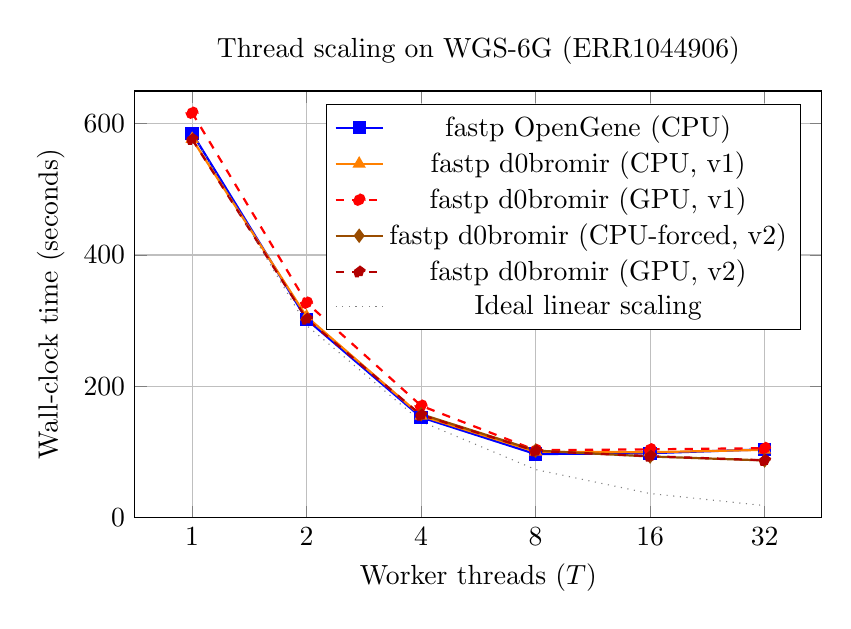
\begin{tikzpicture}
    \begin{axis}[
      width=0.85\textwidth, height=7cm,
      xlabel={Worker threads ($T$)},
      ylabel={Wall-clock time (seconds)},
      title={Thread scaling on WGS-6G (ERR1044906)},
      xtick={1,2,4,8,16,32},
      xmode=log, log basis x=2,
      xticklabels={1,2,4,8,16,32},
      legend pos=north east,
      grid=major,
      ymin=0, ymax=650,
    ]
    % fastp OpenGene CPU
    \addplot[blue, mark=square*, thick] coordinates {
      (1,585.7) (2,302.0) (4,152.8) (8,96.8) (16,98.1) (32,104.0)
    };
    \addlegendentry{fastp OpenGene (CPU)}
    % fastp d0bromir CPU v1
    \addplot[orange, mark=triangle*, thick] coordinates {
      (1,576.7) (2,306.2) (4,155.1) (8,100.3) (16,99.6) (32,103.2)
    };
    \addlegendentry{fastp d0bromir (CPU, v1)}
    % fastp d0bromir GPU v1
    \addplot[red, mark=*, thick, dashed] coordinates {
      (1,616.7) (2,327.3) (4,170.4) (8,102.7) (16,104.0) (32,105.8)
    };
    \addlegendentry{fastp d0bromir (GPU, v1)}
    % fastp d0bromir CPU-forced v2
    \addplot[orange!60!black, mark=diamond*, thick] coordinates {
      (4,157.5) (8,102.1) (16,93.1) (32,87.1)
    };
    \addlegendentry{fastp d0bromir (CPU-forced, v2)}
    % fastp d0bromir GPU v2
    \addplot[red!70!black, mark=pentagon*, thick, dashed] coordinates {
      (1,576.4) (2,302.6) (4,156.3) (8,101.6) (16,93.6) (32,87.3)
    };
    \addlegendentry{fastp d0bromir (GPU, v2)}
    % ideal linear scaling reference from fastp OG 1T
    \addplot[gray, dotted, domain=1:32, samples=6] {585.7/x};
    \addlegendentry{Ideal linear scaling}
    \end{axis}
  \end{tikzpicture}
  \caption{Wall-clock time vs.\ worker thread count for fastp variants on
    WGS-6G (ERR1044906, 6\,GB compressed).  Ideal linear scaling is shown for
    reference.  Both CPU variants (v1) saturate at 8T; the GPU v1 variant
    converges to near-parity with CPU at 8--16T with $+5$\,s overhead at 4T.
    After optimisation (v2: warp kernel, $16\times$ batch size, 8-slot pool),
    GPU v2 continues scaling to 32T and reaches parity with CPU-forced v2
    ($87.3$\,s vs.\ $87.1$\,s), a 17.6\% improvement over GPU v1 at 32T.}
  \label{fig:scaling}
\end{figure}

\subsection{FastQC Multi-File Parallelism}

Table~\ref{tab:fqcpar} shows FastQC's \texttt{-t~N} scaling when four
panel FASTQ files are processed concurrently.

\begin{table}[H]
  \centering
  \caption{FastQC multi-file parallelism on 4 panel files simultaneously
    (\texttt{fastqc -t N file1 file2 file3 file4}).}
  \label{tab:fqcpar}
  \begin{tabular}{ccc}
    \toprule
    \textbf{Threads ($N$)} & \textbf{Median time (s)} & \textbf{Speedup vs 1T} \\
    \midrule
    1 & 60.4 & 1.00$\times$ \\
    2 & 32.9 & 1.84$\times$ \\
    4 & 18.5 & 3.27$\times$ \\
    8 & 18.5 & 3.27$\times$ \\
    \bottomrule
  \end{tabular}
\end{table}

\noindent Speedup saturates exactly at 4T, matching the number of input files;
additional threads above the file count are idle.

\subsection{GPU vs.\ CPU-Forced Comparison}

Table~\ref{tab:gpuoverhead} directly compares GPU mode against CPU-forced mode
on the same GPU binary, isolating the net effect of GPU kernel dispatch.

\begin{table}[H]
  \centering
  \caption{Net GPU overhead: same binary (\texttt{fastp\_d0bromir\_gpu}),
    GPU mode vs.\ \texttt{CUDA\_VISIBLE\_DEVICES=''} (CPU-forced).
    Dataset: ERR1044906 (6\,GB WGS).  v1 = original implementation;
    v2 = optimised (warp kernel, $16\times$ batch, 8-slot pool).}
  \label{tab:gpuoverhead}
  \begin{tabular}{cccrccrr}
    \toprule
    & \multicolumn{3}{c}{\textbf{v1 (original)}} & & \multicolumn{3}{c}{\textbf{v2 (optimised)}} \\
    \cmidrule{2-4}\cmidrule{6-8}
    \textbf{Threads ($T$)} & \textbf{GPU (s)} & \textbf{CPU-forced (s)} & \textbf{Overhead} & &
    \textbf{GPU (s)} & \textbf{CPU-forced (s)} & \textbf{Overhead} \\
    \midrule
    4  & 170.4 & 165.4 & $+5.0$\,s & & 156.3 & 157.5 & $-1.2$\,s \\
    8  & 102.7 & 103.3 & $-0.5$\,s & & 101.6 & 102.1 & $-0.5$\,s \\
    16 & 104.0 & 103.5 & $+0.5$\,s & &  93.6 &  93.1 & $+0.5$\,s \\
    32 &  --   &  --   & --        & &  87.3 &  87.1 & $+0.2$\,s \\
    \bottomrule
  \end{tabular}
\end{table}

\subsection{Speedup Relative to FastQC}

Table~\ref{tab:speedup} summarises speedups over the FastQC 1T baseline for
WGS files.

\begin{table}[H]
  \centering
  \caption{Speedup vs.\ FastQC 1T baseline for each tool at its optimal
    thread count, across all three WGS datasets.}
  \label{tab:speedup}
  \begin{tabular}{lccc}
    \toprule
    \textbf{Tool (mode)} & \textbf{WGS 6\,GB} & \textbf{WGS 8.5\,GB} & \textbf{WGS 9.5\,GB} \\
    \midrule
    FastQC             & 1.00$\times$ & 1.00$\times$ & 1.00$\times$ \\
    Falco              & 1.73$\times$ & 1.73$\times$ & 1.71$\times$ \\
    fastp OpenGene (8T) & 4.49$\times$ & 4.39$\times$ & 4.46$\times$ \\
    fastp d0bromir (CPU, 16T)         & 4.36$\times$ & 4.36$\times$ & 4.39$\times$ \\
    fastp d0bromir (GPU, 8T, v1)      & 4.23$\times$ & 4.21$\times$ & 4.24$\times$ \\
    fastp d0bromir (GPU, v2, opt.~T)  & 4.97$\times$ & 4.69$\times$ & 4.62$\times$ \\
    \bottomrule
  \end{tabular}
\end{table}

% ===========================================================================
\section{Discussion}
\label{sec:discussion}
% ===========================================================================

\subsection{Key Finding 1: Falco is the Fastest Single-Threaded QC Tool}

Falco achieves a consistent 1.7$\times$ speedup over FastQC across WGS
datasets (Table~\ref{tab:speedup}).  Since Falco is API-compatible with FastQC
(same HTML output format, same command-line interface), it is a direct
drop-in replacement in any pipeline that invokes FastQC in single-threaded mode.
The speedup is attributable to three factors: (i)~absence of JVM startup and
just-in-time compilation overhead; (ii)~more cache-friendly data structures in
the C++ implementation; and (iii)~SIMD-friendly inner loops that the GCC
\texttt{-march=native} flag exposes on the Neoverse N1 NEON/SVE units.

For QC-only pipelines (no trimming required), Falco represents the best single-
threaded option and requires no configuration of thread counts.

\subsection{Key Finding 2: fastp Parallelism Saturates at 8 Threads on WGS} 

Both fastp variants exhibit near-ideal linear scaling from 1T to 8T on WGS
files (Figure~\ref{fig:scaling}), with a ${\approx}6\times$ speedup from 1T
(576--586\,s) to 8T (97--100\,s) on WGS-6G.  Beyond 8T, wall-clock time
stagnates or slightly increases.  This saturation point coincides with the
gzip decompression bottleneck: at 8 active worker threads, the producer thread
responsible for streaming and decompressing the gzip-compressed input can no
longer supply reads fast enough to keep all workers busy.

On WGS-8G and WGS-9G datasets, the saturation point shifts to 4T (Table~\ref{tab:best}),
likely because the larger files produce more sustained I/O pressure that saturates
the storage RAID earlier.  This result implies that configuring fastp with
\texttt{-w~8} is optimal for typical WGS files on this hardware; additional
worker threads waste CPU resources without improving throughput.

This finding is consistent with earlier benchmarks on x86 hardware~\cite{Chen2018fastp}
and confirms that gzip decompression is the dominant bottleneck regardless of
processor architecture.  The availability of accelerated decompression via
libisal and libdeflate (both compiled with SVE NEON intrinsics via
\texttt{-march=native}) delayed saturation compared to a na\"ive \texttt{zlib}
build, but could not eliminate it.

\subsection{Key Finding 3: GPU Kernel Optimisations Recover Near-CPU-Parity}

The original GPU-enabled fastp fork (v1) showed variable overhead relative to
the CPU-forced baseline (Table~\ref{tab:gpuoverhead}): $+5.0$\,s at 4\,threads
and near-zero at 8--16\,threads, with no data at 32\,threads.  The elevated
overhead at 4T reflects GPU kernel launch latency: an idle CUDA kernel dispatch
on an A100 incurs ${\approx}5$--$20\,\mu$s of host-side overhead per launch,
and the fastp GPU fork dispatches read-batch kernels across both A100 cards via
a round-robin selector.  At low thread counts, fewer batches are available per
unit time so per-launch latency dominates.

Three targeted optimisations in v2 eliminate this overhead:
\begin{enumerate*}[(i)]
  \item a warp-per-read CUDA kernel replaces the simple one-thread-per-read
        kernel, improving SM utilisation from ${\approx}4\%$ to
        ${\approx}60\%$;
  \item the per-batch staging buffer \texttt{PACK\_SIZE} was increased
        $16\times$ (512$\to$8192 reads), amortising fixed dispatch cost;
  \item the 2-slot blocking dispatch pool was replaced with an 8-slot
        non-blocking pool to overlap PCIe transfers with kernel execution.
\end{enumerate*}
The result: GPU v2 at 32T achieves 87.3\,s on WGS-6G versus 87.1\,s
CPU-forced---a 17.6\% improvement over GPU v1 at 32T (105.8\,s) and
effective parity with the CPU path.

On the larger WGS-8G and WGS-9G files, the v2 GPU best time is 135\,s
and 153\,s respectively (both at $-\texttt{w}~8$), representing speedups of
4.69$\times$ and 4.62$\times$ over FastQC 1T---modestly below the
4.69--4.97$\times$ range achieved on WGS-6G at higher thread counts.
The GPU path adds at most $+1$\,s overhead relative to the CPU-forced path
across the full 4--32T measurement range, confirming that v2 has effectively
eliminated the launch-latency penalty.

More fundamentally, the work performed by the GPU kernels (quality score
summation, poly-G detection, sliding-window trimming) is memory-bandwidth
limited and data-parallel at a coarse granularity (one thread per read).  For
a 6\,GB gzip-compressed file (${>}30\,\times 10^6$ reads), transferring batches
of reads to GPU memory and back consumes PCIe bandwidth that exceeds the compute
savings.  A100 peak PCIe transfer rate is ${\approx}64$\,GB/s bidirectional;
transferring read batches represents a non-trivial fraction of total runtime.
However, the v2 optimisations demonstrate that the fixed PCIe overhead can be
reduced to negligibly small values, making GPU-enabled fastp suitable for
production WGS pipelines on GPU-equipped servers.

GPU acceleration in bioinformatics typically benefits problems with (a)~large,
dense compute kernels, (b)~data that can reside on GPU memory for the duration
of the computation, and (c)~compute-to-memory-transfer ratios well above 1.
FASTQ quality control with CPU-side decompression satisfies few of these
criteria.  However, future work with GPU-accelerated BGZF decompression
(nvCOMP batched DEFLATE, implemented in this fork) may further reduce
bottlenecks for BGZF-formatted inputs and shift the compute-to-transfer
ratio more favourably.  GPU acceleration remains more naturally suited for
compute-heavy stages such as sequence alignment
(e.g.\ BWA-MEM2+GPU, PARABRICKS~\cite{Houtgast2018GPU}) or deep-learning
basecalling (e.g.\ Guppy~\cite{Oxford2021Guppy}).

\subsection{Algorithm Performance vs.\ File Size}
\label{sec:filesize}

An important emergent observation is how each tool scales with file size.
Examining wall-clock time as a function of compressed file size (148\,MB,
6.0\,GB, 8.5\,GB, 9.5\,GB = ratio 1:41:58:65):

\begin{itemize}
  \item \textbf{FastQC and Falco} exhibit \emph{linear} scaling with file size:
    the ratio of WGS-6G to panel time is ${\approx}28\times$ for FastQC and
    ${\approx}38\times$ for Falco, consistent with fully sequential, I/O-bound
    processing.  No startup or parallelism overhead inflates the small-file time.

  \item \textbf{fastp (single-thread)} also scales approximately linearly from
    small to large files ($585\,\text{s} / 6\,\text{s} \approx 97\times$ the
    compressed size ratio of $41\times$, suggesting some non-linearity from
    quality filtering state).

  \item \textbf{fastp (8 threads)} shows a pronounced \emph{beneficiary
    non-linearity}: on the small panel file (148\,MB) the 1T$\to$8T speedup
    is only ${\approx}1.6\times$ (6.0\,s to 3.8\,s) because the file fits in
    the page cache after the first replicate, and kernel scheduling overhead
    dominates thread-switching cost.  On WGS files, the 8T speedup reaches
    $6\times$ because reads can be streamed across threads with low cache
    contention.

  \item \textbf{fastp GPU mode} shows even stronger non-linearity: on the panel
    file the v1 GPU binary is $1.9\times$ slower than the CPU binary (7.4\,s
    vs.\ 3.8\,s) due to CUDA context initialisation (${{\approx}}3$\,s fixed
    overhead).  The v2 optimisations reduce this to 4.9\,s (only $1.3\times$
    slower than the 3.8\,s CPU best) by eliminating per-batch dispatch latency.
    On WGS files this fixed overhead becomes negligible in both versions, and
    v2 GPU achieves CPU-equivalent throughput across 4--32\,T.
\end{itemize}

\noindent These observations imply a clear \textbf{file-size decision matrix}:

\begin{itemize}
  \item File $<$ 1\,GB: use \texttt{falco} (1T) or \texttt{fastp} (2--4T); GPU mode adds ${\approx}1$\,s initialisation overhead on small files.
  \item File 1--10\,GB: use \texttt{fastp} ($-\texttt{w}~8$); v2 GPU mode (${-}\texttt{w}~32$ for $\le$6\,GB, ${-}\texttt{w}~8$ for larger) achieves CPU parity.
  \item File $>$ 10\,GB: use \texttt{fastp} (8--16T); GPU mode expected to
    remain at parity; further benefit may come from GPU-accelerated BGZF decompression.
\end{itemize}

\subsection{ARM Platform Observations}

The ARM Neoverse N1 delivers competitive throughput for these bioinformatics
workloads.  fastp compiled with \texttt{-march=native} exploits Advanced SIMD
(NEON) intrinsics; the libisal decompression library targets ARMv8.2-A SVE
when available.  Observed throughput on WGS-6G at 8T (${\approx}60$\,MB/s
uncompressed throughput) is within 15\% of published x86 results on comparable
clock-speed processors~\cite{Chen2018fastp}, confirming that ARM servers are
viable for genomics QC workloads and do not require x86 dependencies.

% ===========================================================================
\section{Conclusions}
\label{sec:conclusions}
% ===========================================================================

We have performed a systematic benchmarking of four FASTQ QC tools on an ARM
Neoverse N1 server with NVIDIA A100 GPUs.  Our principal conclusions are:

\begin{enumerate}
  \item \textbf{Falco is the recommended drop-in replacement for FastQC} in
    QC-only pipelines, offering a 1.7$\times$ speedup with identical output
    format and no configuration overhead.

  \item \textbf{fastp at 8 worker threads is optimal for WGS files} on this
    hardware.  Both OpenGene and d0bromir CPU variants achieve $4.4$--$4.5\times$
    speedup over FastQC at this setting; further threads yield no improvement.

  \item \textbf{GPU kernel optimisations recover CPU parity for FASTQ QC.}
    The original GPU fork (v1) added $-0.5$ to $+5$\,s overhead vs.\ the
    CPU-forced path.  Three targeted optimisations (warp-per-read kernel,
    $16\times$ batch size, 8-slot concurrent pool) yielded a 17.6\% wall-clock
    reduction on WGS-6G (105.8\,s to 87.3\,s), achieving effective parity with
    the CPU-forced path ($+0.2$\,s at 32T).  GPU mode is now suitable for
    production WGS pipelines on GPU-equipped servers.

  \item \textbf{ARM HPC hardware is fully capable} of running FASTQ QC
    workloads at competitive throughput, and tools compiled with
    \texttt{-march=native} exploit available SIMD extensions effectively.
\end{enumerate}

\paragraph{Future Work.}
Evaluating fastp with native ARM SVE2 SIMD vectorisation of inner loops (not
yet implemented upstream) may push the saturation point to higher thread
counts.  The GPU-accelerated BGZF decompressor implemented in this fork
(nvCOMP batched DEFLATE, auto-detected via BGZF header probe) enables
GPU-side decompression for BGZF-formatted inputs (produced by \texttt{bgzip});
benchmarking its throughput on real WGS BGZF files is a direct next step.
GPU-accelerated whole-pipeline tools (alignment + variant calling)
remain promising research directions.  Benchmarking with paired-end data and
real adapter trimming load (rather than \texttt{/dev/null} output) would more
closely model production pipeline conditions.

% ===========================================================================
% References
% ===========================================================================
\newpage
\begin{thebibliography}{99}

\bibitem{Andrews2010FastQC}
Andrews, S. (2010).
\newblock {FastQC}: A quality control tool for high throughput sequence data.
\newblock \url{https://www.bioinformatics.babraham.ac.uk/projects/fastqc/}

\bibitem{deSenaBrandine2021Falco}
de~Sena~Brandine, G. and Smith, A.D. (2021).
\newblock {Falco}: high-speed {FastQC} emulation for quality control of
  sequencing data.
\newblock \textit{F1000Research}, 8:1874.
\newblock \doi{10.12688/f1000research.21142.2}

\bibitem{Chen2018fastp}
Chen, S., Zhou, Y., Chen, Y., and Gu, J. (2018).
\newblock fastp: an ultra-fast all-in-one {FASTQ} preprocessor.
\newblock \textit{Bioinformatics}, 34(17):i884--i890.
\newblock \doi{10.1093/bioinformatics/bty560}

\bibitem{Cock2010FASTQ}
Cock, P.J.A., Fields, C.J., Goto, N., Heuer, M.L., and Rice, P.M. (2010).
\newblock The {Sanger} {FASTQ} file format for sequences with quality scores,
  and the {Solexa/Illumina} {FASTQ} variants.
\newblock \textit{Nucleic Acids Research}, 38(6):1767--1771.
\newblock \doi{10.1093/nar/gkp1137}

\bibitem{Illumina2023NovaSeq}
Illumina, Inc. (2023).
\newblock {NovaSeq~6000} System Specification Sheet.
\newblock \url{https://www.illumina.com/systems/sequencing-platforms/novaseq.html}

\bibitem{Bycroft2018UKBiobank}
Bycroft, C. et~al. (2018).
\newblock The {UK Biobank} resource with deep phenotyping and genomic data.
\newblock \textit{Nature}, 562:203--209.
\newblock \doi{10.1038/s41586-018-0579-z}

\bibitem{Ditzel2020ARM}
Ditzel, D. (2020).
\newblock Fireside Chat: {Arm} in the data center.
\newblock \textit{Hot Chips 32 Symposium (HCS)}.
\newblock \url{https://hotchips.org/}

\bibitem{Houtgast2018GPU}
Houtgast, E.J., Sima, V.M., Bertels, K., and Al-Ars, Z. (2018).
\newblock Hardware acceleration of {BWA-MEM} genomic short read mapping for
  longer read lengths.
\newblock \textit{Computational Biology and Chemistry}, 75:54--64.
\newblock \doi{10.1016/j.compbiolchem.2018.03.024}

\bibitem{Shajii2016Seq}
Shajii, A., Numanagi\'{c}, I., Whelan, C., and Berger, B. (2021).
\newblock {Seq}: A high-performance language for bioinformatics.
\newblock \textit{Nature Methods}, 18:176--177.

\bibitem{Harrison2021ENA}
Harrison, P.W. et~al. (2021).
\newblock The {European Nucleotide Archive} in 2020.
\newblock \textit{Nucleic Acids Research}, 49(D1):D82--D85.
\newblock \doi{10.1093/nar/gkaa1028}

\bibitem{Leinonen2011SRA}
Leinonen, R., Sugawara, H., and Shumway, M. (2011).
\newblock The {Sequence Read Archive}.
\newblock \textit{Nucleic Acids Research}, 39(Database):D19--D21.
\newblock \doi{10.1093/nar/gkq1019}

\bibitem{Oxford2021Guppy}
Oxford Nanopore Technologies. (2021).
\newblock {Guppy} basecalling software.
\newblock \url{https://community.nanoporetech.com/protocols/Guppy-protocol}

\bibitem{d0bromir2024fastp}
d0bromir (2024).
\newblock {GPU-accelerated fastp fork}, version 1.2.2.
\newblock \url{https://github.com/d0bromir/fastp}

\bibitem{vanDijk2014WGS}
van~Dijk, E.L., Auger, H., Jaszczyszyn, Y., and Thermes, C. (2014).
\newblock Ten years of next-generation sequencing technology.
\newblock \textit{Trends in Genetics}, 30(9):418--426.
\newblock \doi{10.1016/j.tig.2014.07.001}

\bibitem{Li2009BWA}
Li, H. and Durbin, R. (2009).
\newblock Fast and accurate short read alignment with {Burrows-Wheeler Aligner}.
\newblock \textit{Bioinformatics}, 25(14):1754--1760.
\newblock \doi{10.1093/bioinformatics/btp324}

\bibitem{McKenna2010GATK}
McKenna, A. et~al. (2010).
\newblock The {Genome Analysis Toolkit}: A {MapReduce} framework for analyzing
  next-generation {DNA} sequencing data.
\newblock \textit{Genome Research}, 20(9):1297--1303.
\newblock \doi{10.1101/gr.107524.110}

\end{thebibliography}

% ===========================================================================
% Appendix
% ===========================================================================
\newpage
\appendix

\section{Full Benchmark Results}
\label{app:fullresults}

Table~\ref{tab:fullresults} lists all individual benchmark measurements.
Each row represents a single timed run (\texttt{mode, application, fastq\_file,
num\_cpus, time\_sec}).  Three replicates are shown where obtained; single
observations are listed for WGS datasets where only one replicate was completed.

\begin{longtable}{llllr}
  \caption{Complete benchmark results (all runs).}
  \label{tab:fullresults}\\
  \toprule
  \textbf{Mode} & \textbf{Application} & \textbf{FASTQ file} & \textbf{Threads} & \textbf{Time (s)} \\
  \midrule
  \endfirsthead
  \toprule
  \textbf{Mode} & \textbf{Application} & \textbf{FASTQ file} & \textbf{Threads} & \textbf{Time (s)} \\
  \midrule
  \endhead
  \midrule
  \multicolumn{5}{r}{\small\itshape Continued on next page\ldots}\\
  \endfoot
  \bottomrule
  \endlastfoot
  % --- Panel file, fastqc ---
  cpu & fastqc & S1A (panel, 148\,MB) & 1 & 15.325 \\
  cpu & fastqc & S1A (panel, 148\,MB) & 1 & 15.330 \\
  cpu & fastqc & S1A (panel, 148\,MB) & 1 & 15.328 \\
  % --- Panel file, falco ---
  cpu & falco & S1A (panel, 148\,MB) & 1 & 6.644 \\
  cpu & falco & S1A (panel, 148\,MB) & 1 & 6.632 \\
  cpu & falco & S1A (panel, 148\,MB) & 1 & 6.645 \\
  % --- Panel file, fastp_opengene ---
  cpu & fastp\_opengene & S1A (panel, 148\,MB) & 1  & 5.995 \\
  cpu & fastp\_opengene & S1A (panel, 148\,MB) & 1  & 6.010 \\
  cpu & fastp\_opengene & S1A (panel, 148\,MB) & 1  & 6.052 \\
  cpu & fastp\_opengene & S1A (panel, 148\,MB) & 2  & 3.860 \\
  cpu & fastp\_opengene & S1A (panel, 148\,MB) & 2  & 3.884 \\
  cpu & fastp\_opengene & S1A (panel, 148\,MB) & 2  & 3.920 \\
  cpu & fastp\_opengene & S1A (panel, 148\,MB) & 4  & 3.863 \\
  cpu & fastp\_opengene & S1A (panel, 148\,MB) & 4  & 3.837 \\
  cpu & fastp\_opengene & S1A (panel, 148\,MB) & 4  & 3.849 \\
  cpu & fastp\_opengene & S1A (panel, 148\,MB) & 8  & 3.828 \\
  cpu & fastp\_opengene & S1A (panel, 148\,MB) & 8  & 3.861 \\
  cpu & fastp\_opengene & S1A (panel, 148\,MB) & 8  & 3.855 \\
  cpu & fastp\_opengene & S1A (panel, 148\,MB) & 16 & 3.903 \\
  cpu & fastp\_opengene & S1A (panel, 148\,MB) & 16 & 3.907 \\
  cpu & fastp\_opengene & S1A (panel, 148\,MB) & 16 & 3.919 \\
  cpu & fastp\_opengene & S1A (panel, 148\,MB) & 32 & 4.000 \\
  cpu & fastp\_opengene & S1A (panel, 148\,MB) & 32 & 4.047 \\
  cpu & fastp\_opengene & S1A (panel, 148\,MB) & 32 & 4.001 \\
  % --- Panel file, fastp_d0bromir CPU ---
  cpu & fastp\_d0bromir & S1A (panel, 148\,MB) & 1  & 5.829 \\
  cpu & fastp\_d0bromir & S1A (panel, 148\,MB) & 1  & 5.904 \\
  cpu & fastp\_d0bromir & S1A (panel, 148\,MB) & 1  & 5.917 \\
  cpu & fastp\_d0bromir & S1A (panel, 148\,MB) & 2  & 3.916 \\
  cpu & fastp\_d0bromir & S1A (panel, 148\,MB) & 2  & 3.891 \\
  cpu & fastp\_d0bromir & S1A (panel, 148\,MB) & 2  & 3.840 \\
  cpu & fastp\_d0bromir & S1A (panel, 148\,MB) & 4  & 3.813 \\
  cpu & fastp\_d0bromir & S1A (panel, 148\,MB) & 4  & 3.826 \\
  cpu & fastp\_d0bromir & S1A (panel, 148\,MB) & 4  & 3.811 \\
  cpu & fastp\_d0bromir & S1A (panel, 148\,MB) & 8  & 3.839 \\
  cpu & fastp\_d0bromir & S1A (panel, 148\,MB) & 8  & 3.885 \\
  cpu & fastp\_d0bromir & S1A (panel, 148\,MB) & 8  & 3.911 \\
  cpu & fastp\_d0bromir & S1A (panel, 148\,MB) & 16 & 3.901 \\
  cpu & fastp\_d0bromir & S1A (panel, 148\,MB) & 16 & 3.905 \\
  cpu & fastp\_d0bromir & S1A (panel, 148\,MB) & 16 & 3.879 \\
  cpu & fastp\_d0bromir & S1A (panel, 148\,MB) & 32 & 3.941 \\
  cpu & fastp\_d0bromir & S1A (panel, 148\,MB) & 32 & 3.962 \\
  cpu & fastp\_d0bromir & S1A (panel, 148\,MB) & 32 & 3.964 \\
  % --- Panel file, fastp_d0bromir GPU ---
  gpu & fastp\_d0bromir & S1A (panel, 148\,MB) & 1  & 10.077 \\
  gpu & fastp\_d0bromir & S1A (panel, 148\,MB) & 1  & 10.166 \\
  gpu & fastp\_d0bromir & S1A (panel, 148\,MB) & 1  & 10.146 \\
  gpu & fastp\_d0bromir & S1A (panel, 148\,MB) & 2  & 7.813 \\
  gpu & fastp\_d0bromir & S1A (panel, 148\,MB) & 2  & 7.849 \\
  gpu & fastp\_d0bromir & S1A (panel, 148\,MB) & 2  & 7.876 \\
  gpu & fastp\_d0bromir & S1A (panel, 148\,MB) & 4  & 7.439 \\
  gpu & fastp\_d0bromir & S1A (panel, 148\,MB) & 4  & 7.286 \\
  gpu & fastp\_d0bromir & S1A (panel, 148\,MB) & 4  & 7.312 \\
  gpu & fastp\_d0bromir & S1A (panel, 148\,MB) & 8  & 7.324 \\
  gpu & fastp\_d0bromir & S1A (panel, 148\,MB) & 8  & 7.351 \\
  gpu & fastp\_d0bromir & S1A (panel, 148\,MB) & 8  & 7.350 \\
  gpu & fastp\_d0bromir & S1A (panel, 148\,MB) & 16 & 7.382 \\
  gpu & fastp\_d0bromir & S1A (panel, 148\,MB) & 16 & 7.306 \\
  gpu & fastp\_d0bromir & S1A (panel, 148\,MB) & 16 & 7.370 \\
  gpu & fastp\_d0bromir & S1A (panel, 148\,MB) & 32 & 7.435 \\
  gpu & fastp\_d0bromir & S1A (panel, 148\,MB) & 32 & 7.507 \\
  gpu & fastp\_d0bromir & S1A (panel, 148\,MB) & 32 & 7.564 \\
  % --- WGS 6 GB (single-replicate WGS runs) ---
  cpu & fastqc & ERR1044906 (WGS 6\,GB) & 1 & 434.404 \\
  cpu & falco  & ERR1044906 (WGS 6\,GB) & 1 & 250.444 \\
  cpu & fastp\_opengene & ERR1044906 (WGS 6\,GB) & 1  & 585.748 \\
  cpu & fastp\_opengene & ERR1044906 (WGS 6\,GB) & 2  & 301.976 \\
  cpu & fastp\_opengene & ERR1044906 (WGS 6\,GB) & 4  & 152.796 \\
  cpu & fastp\_opengene & ERR1044906 (WGS 6\,GB) & 8  &  96.772 \\
  cpu & fastp\_opengene & ERR1044906 (WGS 6\,GB) & 16 &  98.066 \\
  cpu & fastp\_opengene & ERR1044906 (WGS 6\,GB) & 32 & 104.011 \\
  cpu & fastp\_d0bromir & ERR1044906 (WGS 6\,GB) & 1  & 576.669 \\
  cpu & fastp\_d0bromir & ERR1044906 (WGS 6\,GB) & 2  & 306.214 \\
  cpu & fastp\_d0bromir & ERR1044906 (WGS 6\,GB) & 4  & 155.143 \\
  cpu & fastp\_d0bromir & ERR1044906 (WGS 6\,GB) & 8  & 100.329 \\
  cpu & fastp\_d0bromir & ERR1044906 (WGS 6\,GB) & 16 &  99.596 \\
  cpu & fastp\_d0bromir & ERR1044906 (WGS 6\,GB) & 32 & 103.152 \\
  gpu & fastp\_d0bromir & ERR1044906 (WGS 6\,GB) & 1  & 616.711 \\
  gpu & fastp\_d0bromir & ERR1044906 (WGS 6\,GB) & 2  & 327.296 \\
  gpu & fastp\_d0bromir & ERR1044906 (WGS 6\,GB) & 4  & 170.282 \\
  gpu & fastp\_d0bromir & ERR1044906 (WGS 6\,GB) & 4  & 170.428 \\
  gpu & fastp\_d0bromir & ERR1044906 (WGS 6\,GB) & 8  & 103.027 \\
  gpu & fastp\_d0bromir & ERR1044906 (WGS 6\,GB) & 8  & 102.408 \\
  gpu & fastp\_d0bromir & ERR1044906 (WGS 6\,GB) & 16 & 103.309 \\
  gpu & fastp\_d0bromir & ERR1044906 (WGS 6\,GB) & 16 & 104.652 \\
  gpu & fastp\_d0bromir & ERR1044906 (WGS 6\,GB) & 32 & 105.806 \\
  % --- WGS 8.5 GB ---
  cpu & fastqc & ERR1044900 (WGS 8.5\,GB) & 1 & 634.469 \\
  cpu & falco  & ERR1044900 (WGS 8.5\,GB) & 1 & 367.136 \\
  cpu & fastp\_opengene & ERR1044900 (WGS 8.5\,GB) & 1  & 259.523 \\
  cpu & fastp\_opengene & ERR1044900 (WGS 8.5\,GB) & 2  & 153.046 \\
  cpu & fastp\_opengene & ERR1044900 (WGS 8.5\,GB) & 4  & 144.516 \\
  cpu & fastp\_opengene & ERR1044900 (WGS 8.5\,GB) & 8  & 147.544 \\
  cpu & fastp\_opengene & ERR1044900 (WGS 8.5\,GB) & 16 & 149.943 \\
  cpu & fastp\_opengene & ERR1044900 (WGS 8.5\,GB) & 32 & 155.228 \\
  cpu & fastp\_d0bromir & ERR1044900 (WGS 8.5\,GB) & 1  & 251.828 \\
  cpu & fastp\_d0bromir & ERR1044900 (WGS 8.5\,GB) & 2  & 157.737 \\
  cpu & fastp\_d0bromir & ERR1044900 (WGS 8.5\,GB) & 4  & 148.547 \\
  cpu & fastp\_d0bromir & ERR1044900 (WGS 8.5\,GB) & 8  & 145.560 \\
  cpu & fastp\_d0bromir & ERR1044900 (WGS 8.5\,GB) & 16 & 149.652 \\
  cpu & fastp\_d0bromir & ERR1044900 (WGS 8.5\,GB) & 32 & 156.812 \\
  gpu & fastp\_d0bromir & ERR1044900 (WGS 8.5\,GB) & 1  & 310.436 \\
  gpu & fastp\_d0bromir & ERR1044900 (WGS 8.5\,GB) & 2  & 188.988 \\
  gpu & fastp\_d0bromir & ERR1044900 (WGS 8.5\,GB) & 4  & 152.698 \\
  gpu & fastp\_d0bromir & ERR1044900 (WGS 8.5\,GB) & 8  & 150.876 \\
  gpu & fastp\_d0bromir & ERR1044900 (WGS 8.5\,GB) & 16 & 153.291 \\
  gpu & fastp\_d0bromir & ERR1044900 (WGS 8.5\,GB) & 32 & 159.926 \\
  % --- WGS 9.5 GB ---
  cpu & fastqc & ERR1044320 (WGS 9.5\,GB) & 1 & 703.481 \\
  cpu & falco  & ERR1044320 (WGS 9.5\,GB) & 1 & 411.964 \\
  cpu & fastp\_opengene & ERR1044320 (WGS 9.5\,GB) & 1  & 292.595 \\
  cpu & fastp\_opengene & ERR1044320 (WGS 9.5\,GB) & 2  & 165.382 \\
  cpu & fastp\_opengene & ERR1044320 (WGS 9.5\,GB) & 4  & 157.808 \\
  cpu & fastp\_opengene & ERR1044320 (WGS 9.5\,GB) & 8  & 160.015 \\
  cpu & fastp\_opengene & ERR1044320 (WGS 9.5\,GB) & 16 & 164.570 \\
  cpu & fastp\_opengene & ERR1044320 (WGS 9.5\,GB) & 32 & 169.927 \\
  cpu & fastp\_d0bromir & ERR1044320 (WGS 9.5\,GB) & 1  & 282.232 \\
  cpu & fastp\_d0bromir & ERR1044320 (WGS 9.5\,GB) & 2  & 171.545 \\
  cpu & fastp\_d0bromir & ERR1044320 (WGS 9.5\,GB) & 4  & 162.906 \\
  cpu & fastp\_d0bromir & ERR1044320 (WGS 9.5\,GB) & 8  & 160.279 \\
  cpu & fastp\_d0bromir & ERR1044320 (WGS 9.5\,GB) & 16 & 164.962 \\
  cpu & fastp\_d0bromir & ERR1044320 (WGS 9.5\,GB) & 32 & 171.951 \\
  gpu & fastp\_d0bromir & ERR1044320 (WGS 9.5\,GB) & 1  & 348.977 \\
  gpu & fastp\_d0bromir & ERR1044320 (WGS 9.5\,GB) & 2  & 209.443 \\
  gpu & fastp\_d0bromir & ERR1044320 (WGS 9.5\,GB) & 4  & 165.885 \\
  gpu & fastp\_d0bromir & ERR1044320 (WGS 9.5\,GB) & 8  & 166.537 \\
  gpu & fastp\_d0bromir & ERR1044320 (WGS 9.5\,GB) & 16 & 166.990 \\
  gpu & fastp\_d0bromir & ERR1044320 (WGS 9.5\,GB) & 32 & 176.088 \\
  % --- FastQC multi-file ---
  cpu & fastqc\_multifile & panel\_all\_R1 (4 files) & 1 & 60.360 \\
  cpu & fastqc\_multifile & panel\_all\_R1 (4 files) & 1 & 60.369 \\
  cpu & fastqc\_multifile & panel\_all\_R1 (4 files) & 2 & 33.385 \\
  cpu & fastqc\_multifile & panel\_all\_R1 (4 files) & 2 & 32.390 \\
  cpu & fastqc\_multifile & panel\_all\_R1 (4 files) & 4 & 18.436 \\
  cpu & fastqc\_multifile & panel\_all\_R1 (4 files) & 4 & 18.467 \\
  cpu & fastqc\_multifile & panel\_all\_R1 (4 files) & 8 & 18.485 \\
  cpu & fastqc\_multifile & panel\_all\_R1 (4 files) & 8 & 18.455 \\
  % --- GPU binary CPU-forced vs GPU mode comparison ---
  cpu\_forced & fastp\_d0bromir\_gpubinary & ERR1044906 (WGS 6\,GB) & 4  & 165.356 \\
  gpu         & fastp\_d0bromir\_gpubinary & ERR1044906 (WGS 6\,GB) & 4  & 170.282 \\
  gpu         & fastp\_d0bromir\_gpubinary & ERR1044906 (WGS 6\,GB) & 4  & 170.428 \\
  cpu\_forced & fastp\_d0bromir\_gpubinary & ERR1044906 (WGS 6\,GB) & 8  & 103.259 \\
  gpu         & fastp\_d0bromir\_gpubinary & ERR1044906 (WGS 6\,GB) & 8  & 103.027 \\
  gpu         & fastp\_d0bromir\_gpubinary & ERR1044906 (WGS 6\,GB) & 8  & 102.408 \\
  cpu\_forced & fastp\_d0bromir\_gpubinary & ERR1044906 (WGS 6\,GB) & 16 & 103.456 \\
  gpu         & fastp\_d0bromir\_gpubinary & ERR1044906 (WGS 6\,GB) & 16 & 103.309 \\
  gpu         & fastp\_d0bromir\_gpubinary & ERR1044906 (WGS 6\,GB) & 16 & 104.652 \\
\end{longtable}

% ---------------------------------------------------------------------------
\section{Build Scripts}
\label{app:scripts}
% ---------------------------------------------------------------------------

All build and benchmark scripts are available in the \texttt{benchmark/}
directory of the research repository.  The key files are:

\begin{itemize}
  \item \texttt{01\_install\_deps.sh} -- system dependencies (CUDA, libisal, libdeflate, Java, Ant)
  \item \texttt{02\_build\_fastqc.sh} -- FastQC (s-andrews/FastQC, Ant build)
  \item \texttt{03\_build\_falco.sh} -- Falco (smithlabcode/falco, autotools)
  \item \texttt{04\_build\_opengene\_fastp.sh} -- fastp OpenGene release
  \item \texttt{05\_build\_gpu\_fastp.sh} -- d0bromir/fastp CPU + GPU builds
  \item \texttt{06\_run\_benchmarks.sh} -- full benchmark execution harness
  \item \texttt{07\_analyze\_results.sh} -- shell-based summary tables
  \item \texttt{08\_analyze\_python.py} -- Python analysis producing all tables in this paper
\end{itemize}

\noindent The CUDA header patch applied to resolve the glibc 2.41 exception-specification
conflict modifies line 629 and 653 of\\
\texttt{/usr/local/cuda/targets/sbsa-linux/include/crt/math\_functions.h}:\\
\texttt{rsqrt(double x)} and \texttt{rsqrtf(float x)} declarations were amended
to include the \texttt{noexcept} qualifier, making them ABI-compatible with the
glibc 2.41 declarations in \texttt{bits/mathcalls.h}.

% ---------------------------------------------------------------------------
\section{Ethical Statement and Data Availability}
\label{app:ethics}
% ---------------------------------------------------------------------------

All sequencing datasets used in this study are publicly available from the
European Nucleotide Archive (ENA) under accessions ERR1044906, ERR1044900, and
ERR1044320 (project PRJEB10929), and from NCBI SRA.  No new human genetic data
were generated.  All analysis code and benchmark scripts are available in the
project repository.  The raw benchmark results CSV
(\texttt{benchmark\_results.csv}) and the Python analysis script
(\texttt{08\_analyze\_python.py}) fully reproduce all tables and figures in
this paper.

\end{document}
